\chapter{Shadow Dexterous Hand - Technical Specifications}\label{app:shadow-dexterous-hand-technical-specifications}

\tabref{app:range-of-motion-shadow-hand} shows the \gls{rom} for the Shadow Dexterous Hand and \tabref{app:range-of-motion-human-hand} shown the \gls{rom} for a human hand. The shorthand abbreviations used in these tables can be seen listed in \tabref{app:joint-abbreviations}. The joints are numbered from fingertip to base and thus FF1 refers to the first joint after the fingertip on the first finger i.e. the index finger.
\begin{table}[!h]
\begin{center}
	\begin{tabular}{ |p{0.22\textwidth}|p{0.08\textwidth}|p{0.08\textwidth}|p{0.08\textwidth}|p{0.08\textwidth}|p{0.3\textwidth}| } 
	\hline
	\multicolumn{6}{|c|}{\textbf{\gls{rom} - Shadow Dexterous Hand}} \\ \hline
	\textbf{Joint(s)} & \textbf{Min deg} & \textbf{Max deg} & \textbf{Min rad} & \textbf{Max rad} & \textbf{Notes} \\ \hline
	FF1, MF1, RF1, LF1 &0&90&0&1.571  & \multirow{2}{4em}{Coupled}\\ \cline{1-5}
	FF2, MF2, RF2, LF2 & 0   & 90 & 0      & 1.571 & \\ \hline
	FF3, MF3, RF3, LF3 & -15 & 90 & -0.262 & 1.571 & \\ \hline
	FF4, MF4, RF4, LF4 & -20 & 20 & -0.349 & 0.349 & \\ \hline
	LF5&0&45&0&0.785 &  \\ \hline
	TH1&-15&90&-0.262&1.571 &  \\ \hline
	TH2&-40&40&-0.698&0.698 &  \\ \hline
	TH3&-12&12&-0.209&0.209 &  \\ \hline
	TH4&0&70&0&1.222& \\ \hline
	TH5&-60&60&-1.047&1.047& \\ \hline
	WR1&-40&28&-0.698&0.489& \\ \hline
	WR2&-28&10&-0.489&0.174& \\ \hline
	\end{tabular}
	\caption{The ranges of motion for each joint in the Shadow Dexterous Hand~\cite{range-of-motion-shadow-hand}.}
	\label{app:range-of-motion-shadow-hand}
\end{center}
\end{table}

\begin{table}[!h]
	\begin{center}
		\begin{tabular}{ |p{0.22\textwidth}|p{0.08\textwidth}|p{0.08\textwidth}|p{0.08\textwidth}|p{0.08\textwidth}|p{0.3\textwidth}| } 
		\hline
		\multicolumn{6}{|c|}{\textbf{\gls{rom} - Human Hand}} \\ \hline
		\textbf{Joint(s)} & \textbf{Min deg} & \textbf{Max deg} & \textbf{Min rad} & \textbf{Max rad} & \textbf{Latin Name} \\ \hline
		TH1 & -15 & 80 & & & Interphalangeal (IP) \\ \hline
		TH2 + TH3 & -10 & 55 & & & Metacarpophalangeal (MCP)\\ \hline
		TH4 +TH5  & -10 & 55 & & & Carpometacarpal (CMC)\\ \hline
		FF1, MF1, RF1, LF1 & 0 & 80 & & & Distal interphalangeal (DIP) \\ \hline
		FF2, MF2, RF2, LF2 & 0 & 100 & & & Proximal interphalangeal (PIP) \\ \hline
		FF3, MF3, RF3, LF3 & -45 & 90 & & & Metacarpophalangeal (MCP) \\ \hline
		WR1 &-80&80& & & Radiocarpal \\ \hline
		WR2 &-28&20& & & Radiocarpal \\ \hline
		\end{tabular}
		\caption{The theoretical \gls{rom} for each finger joint in human hand~\cite{continuous-and-simultaneous-estimation-of-finger-kinematics-using-inputs-from-an-emg-to-muscle-activation-model} and found \gls{rom} for the wrist joints~\cite{functional-wrist-motion:-a-biomechanical-study}.}
		\label{app:range-of-motion-human-hand}
	\end{center}
\end{table}

\begin{table}[!h]
	\begin{center}
		\begin{tabular}{ |l|l| } 
		\hline
		\multicolumn{2}{|c|}{\textbf{Joint Name Abbreviation}} \\ \hline
		\textbf{Abbreviation} & \textbf{Full Name} \\ \hline
		FF & First Finger \\ \hline 
		MF & Middle Finger \\ \hline 
		RF & Ring Finger \\ \hline 
		LF & Little Finger \\ \hline 
		WR & Wrist \\ \hline 
		\end{tabular}
		\caption{The abbreviations used to reference ~\cite{joint-abbreviations-shadow-hand}.}
		\label{app:joint-abbreviations}
	\end{center}
	\end{table}

To compare the kinematic structure of the Shadow Dexterous Hand and a human hand, see~\figref{app:human-and-robot-hand-kinematics}.

\begin{figure}[!h]
	\centering
	\begin{subfigure}[b]{0.3\textwidth}
		\centering
		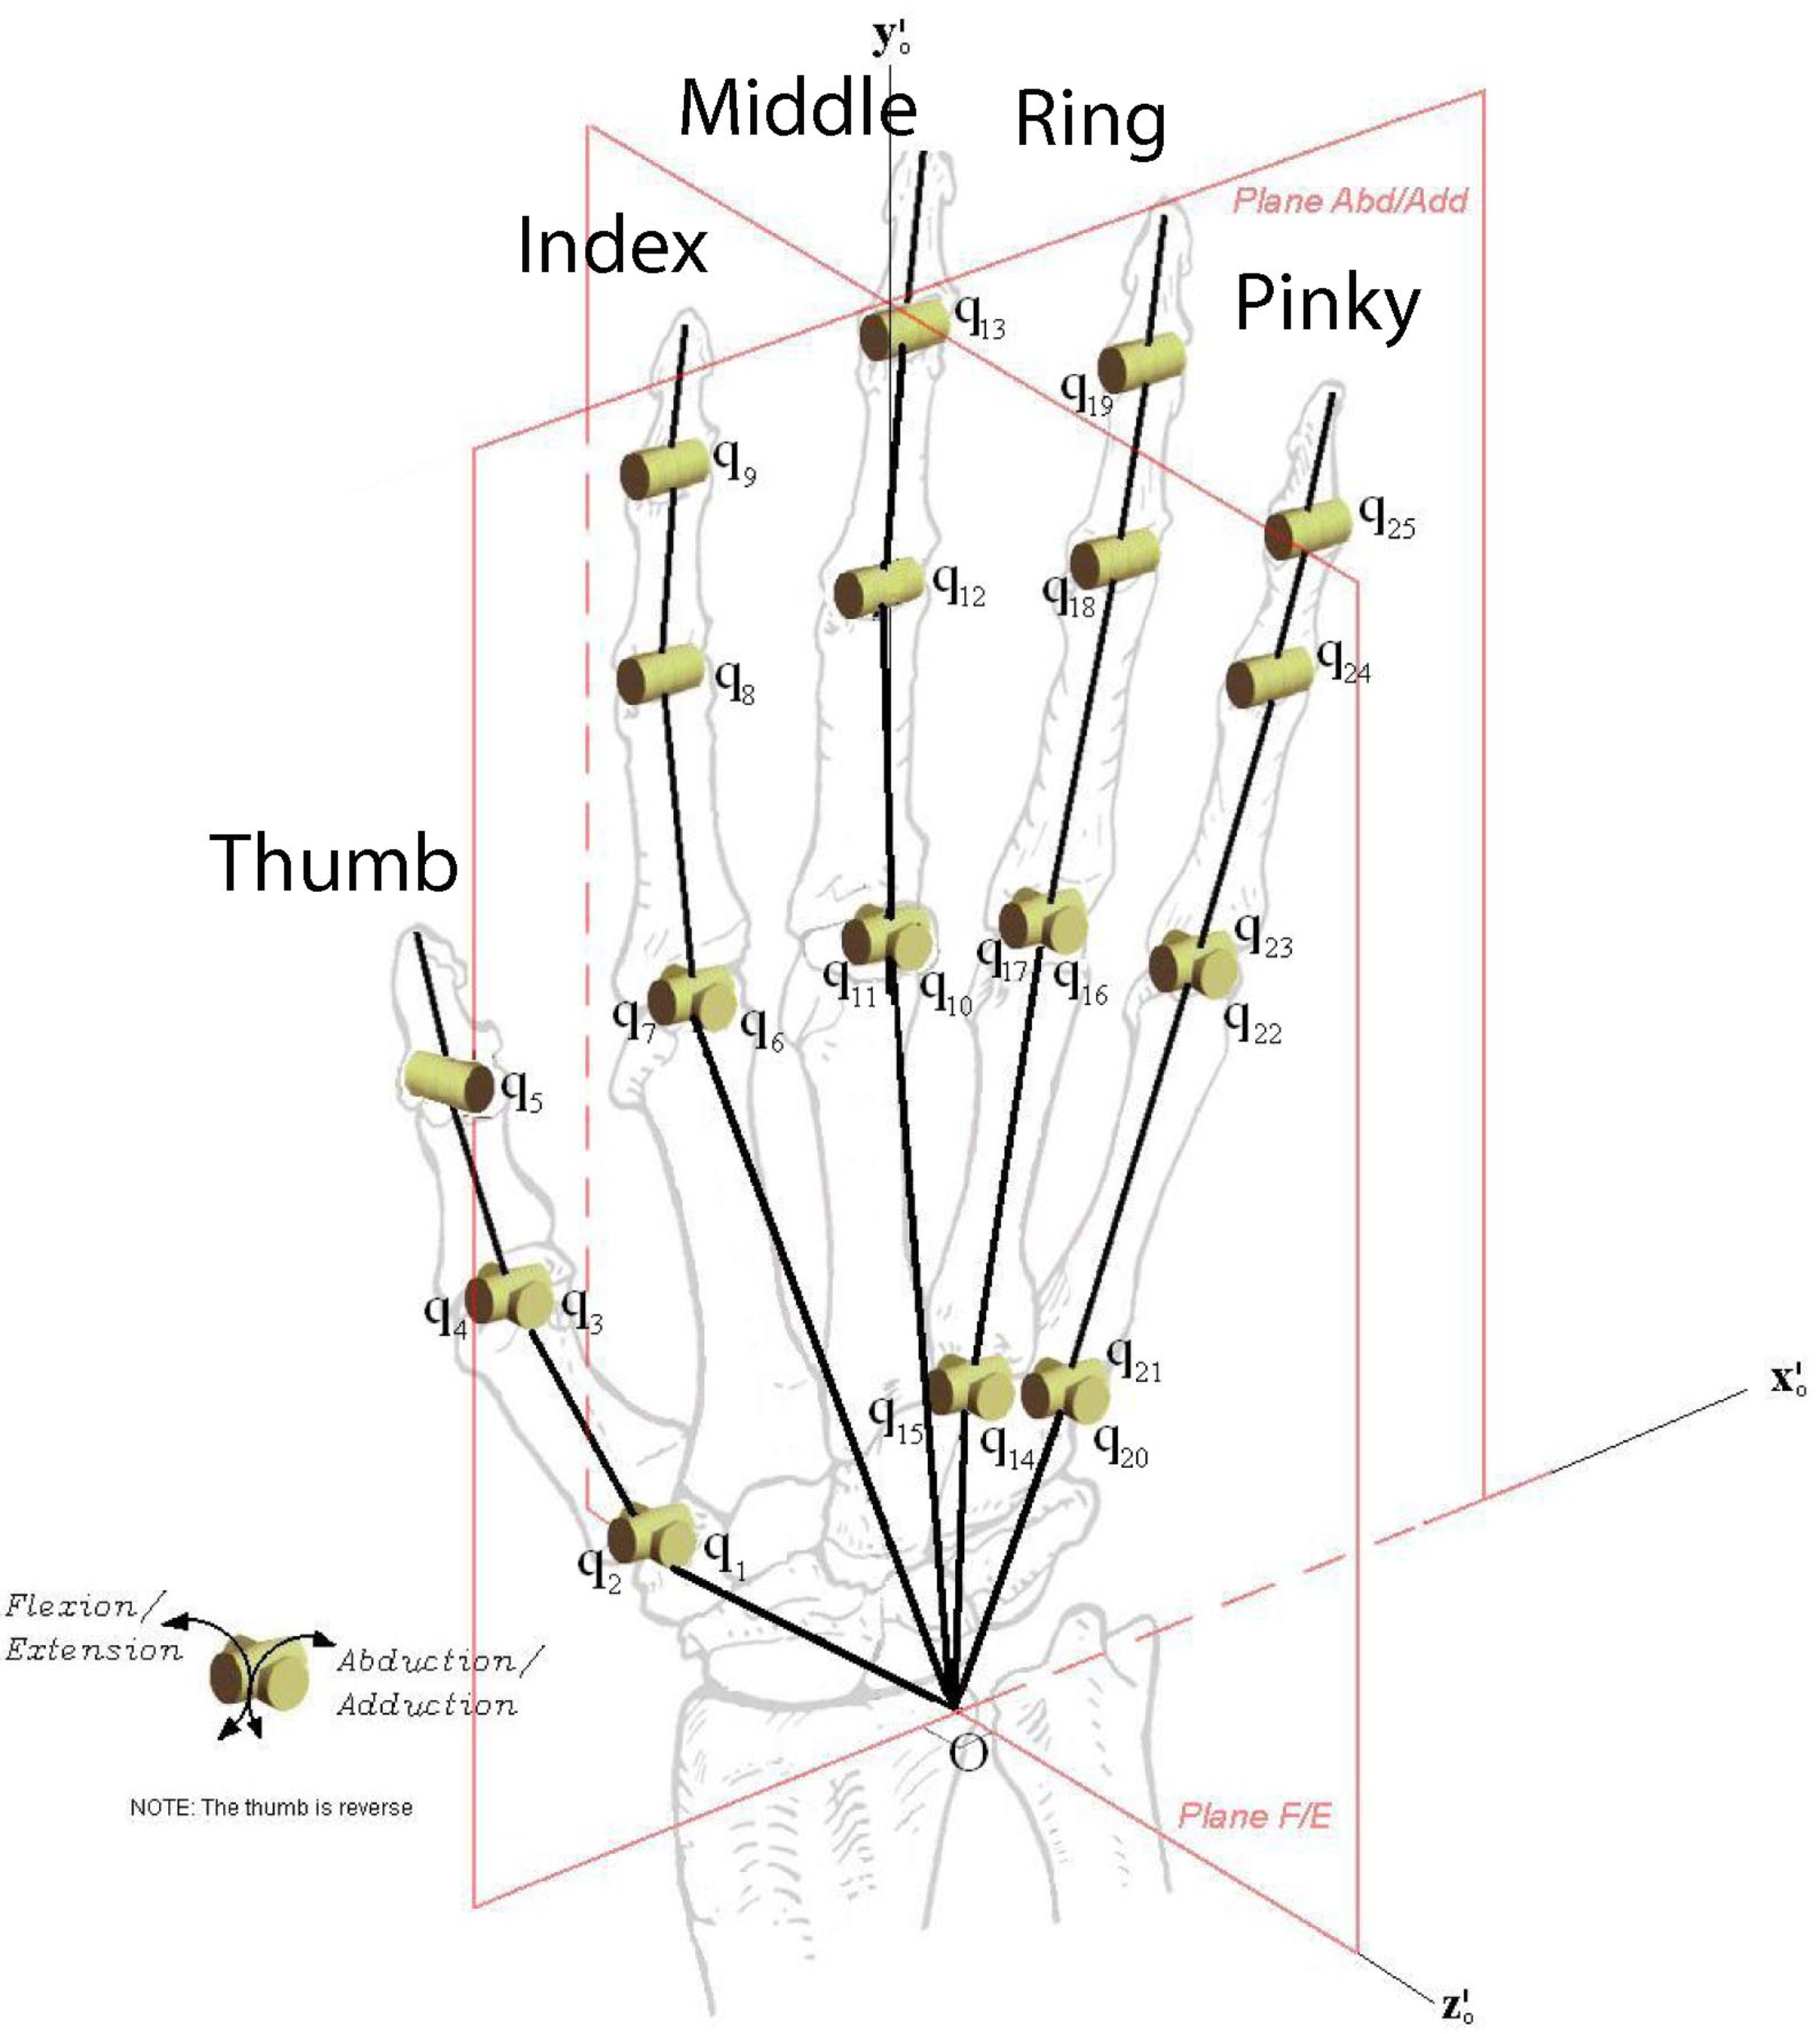
\includegraphics[width=\textwidth]{chapters/appendix/fig/human-hand-kinematics.pdf}
		\caption{The kinematic tree of a human hand according to~\cite{grasp-synthesis-algorithms-for-multifingered-robot-hands}.}
		\label{app:human-hand-kinematics}
	\end{subfigure}
	\hfill
	\begin{subfigure}[b]{0.69\textwidth}
		\centering
		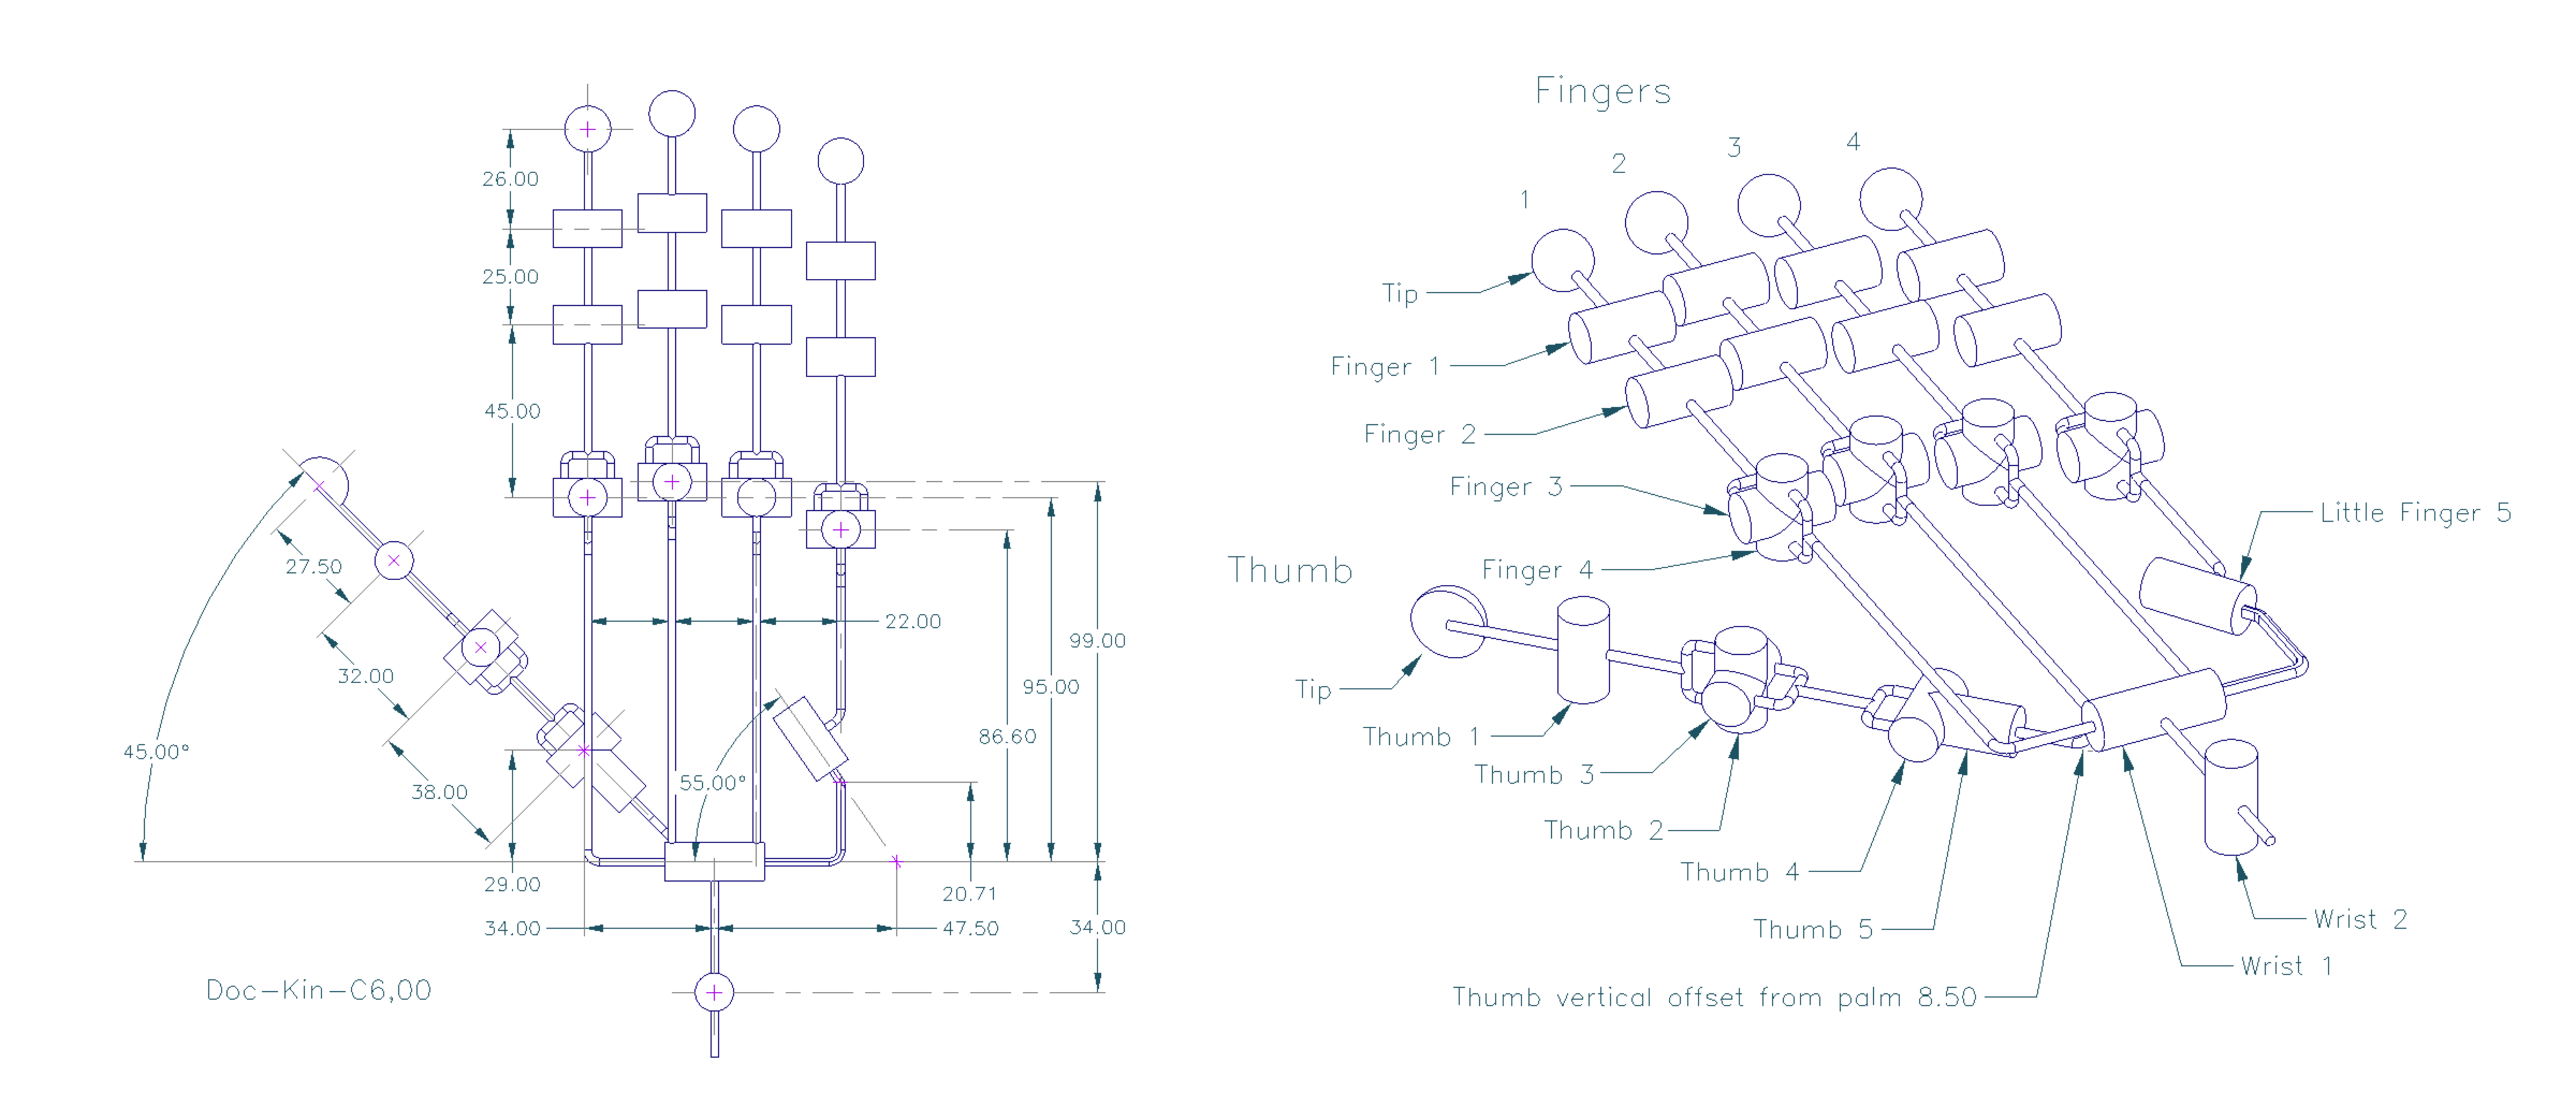
\includegraphics[width=\textwidth]{chapters/appendix/fig/robot-hand-kinematics.pdf}
		\caption{The kinematic tree of the Shadow Dexterous Hand according to~\cite{robot-hand-kinematics}. \newline}
		\label{app:robot-hand-kinematics}
	\end{subfigure}
	\caption{The kinematic trees of a human hand and the Shadow Dexterous hand.}
	\label{app:human-and-robot-hand-kinematics}
\end{figure}

\chapter{Tactile Perception - Simulated Electrode Activations}\label{app:tactile-perception-simulated-electrode-activations}

Below three 

\begin{figure}[!h]
	\begin{center}
		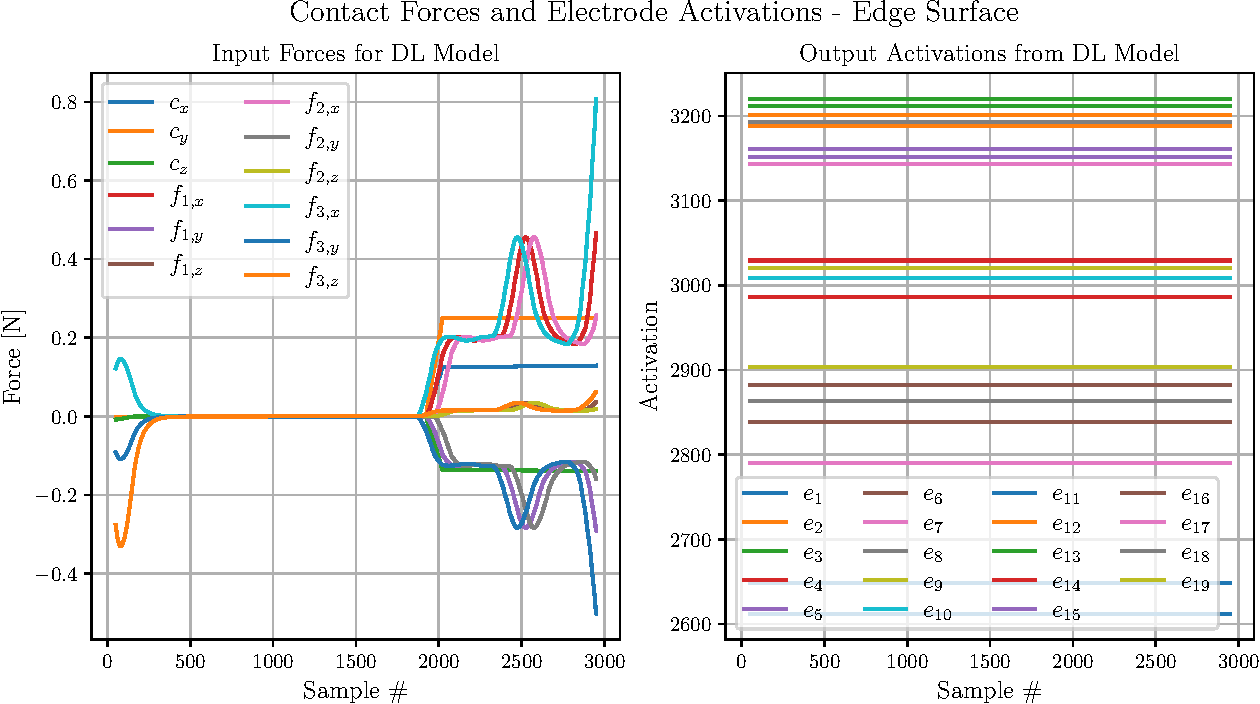
\includegraphics[width=\textwidth]{chapters/1-tactile-perception/fig/matplotlib/edge-contact-graph.pdf}
	\end{center}
	\caption{he simulated tactile electrode activations when the simulated Shadow Dexterous hand's index finger is in contact with an edge.}
	\label{app:edge-contact-graph}
\end{figure}

\begin{figure}[!h]
	\begin{center}
		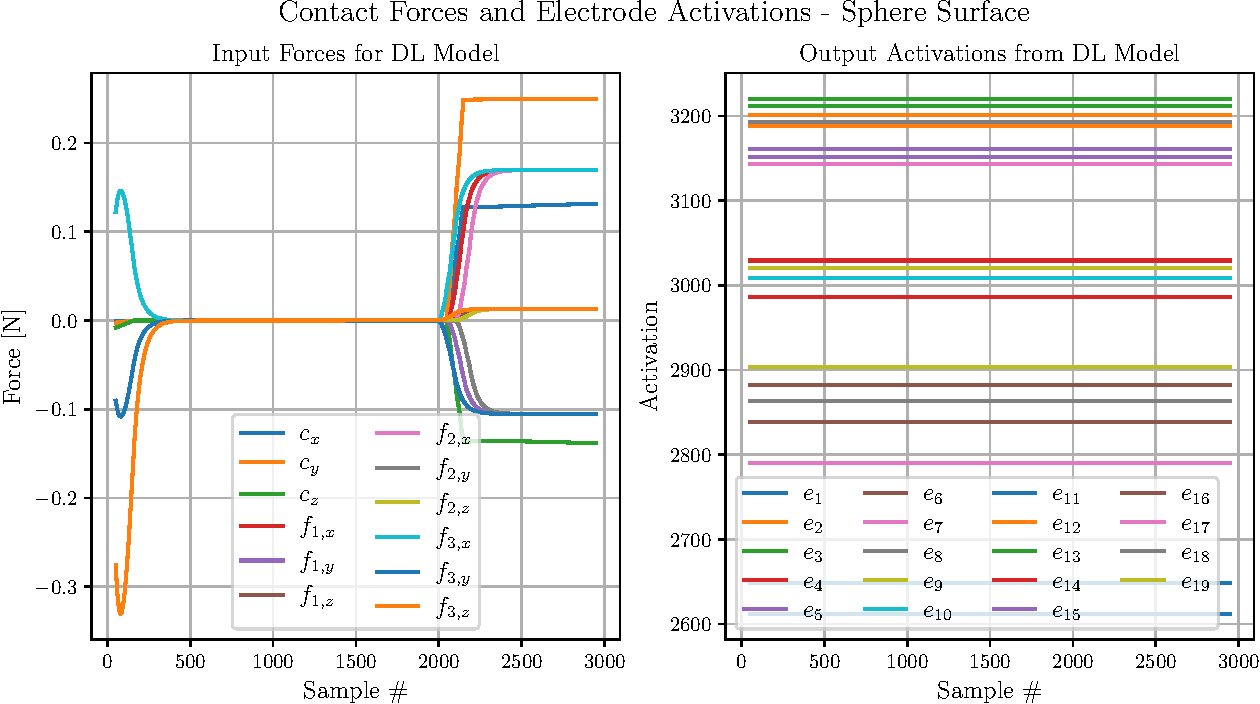
\includegraphics[width=\textwidth]{chapters/1-tactile-perception/fig/matplotlib/sphere-contact-graph.pdf}
	\end{center}
	\caption{The simulated tactile electrode activations when the simulated Shadow Dexterous hand's index finger is in contact with a smooth surface.}
	\label{app:smooth-contact-graph}
\end{figure}

\begin{figure}[!h]
	\begin{center}
		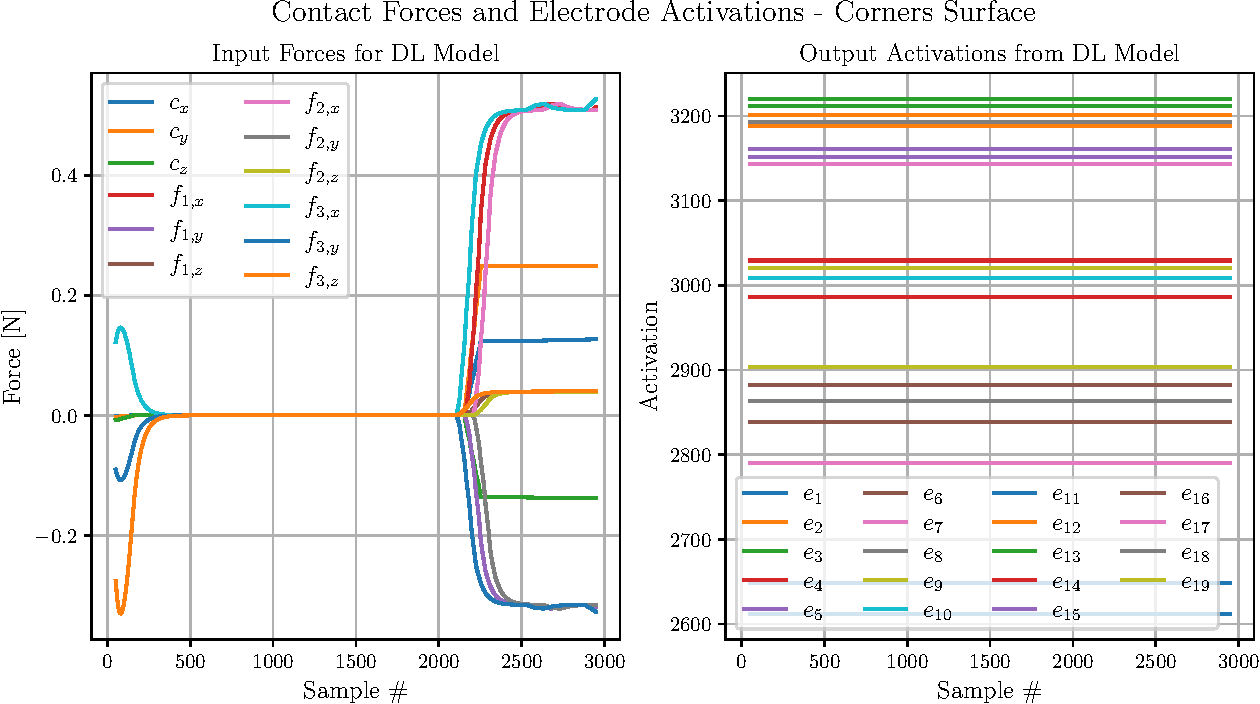
\includegraphics[width=\textwidth]{chapters/1-tactile-perception/fig/matplotlib/corners-contact-graph.pdf}
	\end{center}
	\caption{The simulated tactile electrode activations when the simulated Shadow Dexterous hand's index finger is in contact with a corner.}
	\label{app:corner-contact-graph}
\end{figure}